\documentclass{article}
\usepackage{listings}
\usepackage{xcolor}
\usepackage{subcaption}
\usepackage{hyperref}
\usepackage{blindtext}
\usepackage{geometry}
\usepackage{graphicx}
\usepackage{wrapfig}
 \geometry{
 a4paper,
 total={170mm,257mm},
 left=20mm,
 top=20mm,
 }
\hypersetup{
    colorlinks=true,
    linkcolor=blue,
    filecolor=magenta,      
    urlcolor=cyan,
    pdftitle={Overleaf Example},
    pdfpagemode=FullScreen,
    }

\urlstyle{same}

\definecolor{codegreen}{rgb}{0,0.6,0}
\definecolor{codegray}{rgb}{0.5,0.5,0.5}
\definecolor{codepurple}{rgb}{0.58,0,0.82}
\definecolor{backcolour}{rgb}{0.95,0.95,0.92}

\lstdefinestyle{mystyle}{
    backgroundcolor=\color{backcolour},   
    commentstyle=\color{codegreen},
    keywordstyle=\color{magenta},
    numberstyle=\tiny\color{codegray},
    stringstyle=\color{codepurple},
    basicstyle=\ttfamily\footnotesize,
    breakatwhitespace=false,         
    breaklines=true,                 
    captionpos=b,                    
    keepspaces=true,                 
    numbers=left,                    
    numbersep=5pt,                  
    showspaces=false,                
    showstringspaces=false,
    showtabs=false,                  
    tabsize=2
}
\lstset{style=mystyle}

\graphicspath{ {./images/} }






\title{\textbf{Customer Satisfaction Prediction using Python and Machine Learning(CP-08)}}
\author{Sani Anna Varghese , Jobin Pius and Christo Joseph Sajan}
\date{\textit{Saintgits Group of Institutions, Kottayam, Kerala}}

\begin{document}
\begin{figure}[t]
\includegraphics[width=2cm]{Picture.png}

\end{figure}
\maketitle


\section{Abstract}
This report underscores the vital role of customer satisfaction in modern busi- ness and explores advanced strategies for enhancement. Leveraging machine learning, businesses predict and address satisfaction proactively, driving can retention, loyalty, and competitiveness. Analysis of survey data identifies key satisfaction factors for targeted improvements. Prioritizing satisfaction leads to actionable strategies outlined in the report, crucial for business success in to- day's market. By implementing these strategies, companies can achieve tangible improvements in customer satisfaction, retention, and overall business perfor- mance, ensuring a strong position in the competitive landscape.

\section{Introduction}
In the contemporary business landscape, customer satisfaction stands as a cornerstone of success, shaping consumer preferences, loyalty, and market competitiveness. This paper navigates through the pivotal role that customer satisfaction plays in driving modern business strategies and explores innovative methodologies to bolster it further. With the advent of machine learning technologies, businesses now possess the capability to anticipate and address customer satisfaction proactively, thereby fostering enhanced retention rates, brand loyalty, and a stronger foothold in the market.
By delving into survey data analysis, companies can unveil crucial insights into the factors that significantly influence customer satisfaction, empowering targeted enhancements in their offerings. The prioritization of customer satisfaction emerges not only as a strategic imperative but as a fundamental driver of sustained business success amidst evolving consumer demands and fierce market competition.
This paper aims to delineate actionable strategies derived from the primacy of customer satisfaction, equipping businesses with the requisite tools to drive measurable improvements in customer retention, loyalty, and overall organizational performance. Through the effective implementation of these strategies, companies can fortify their market positioning and navigate the competitive landscape with confidence and resilience.
\section{Literature Review}
To kickstart our project and devise an optimal methodology for modeling and data processing, we've scoured various papers and blogs. These resources pro- vide valuable insights into crafting effective models tailored to our dataset. Since this is a good dataset there were plenty of works for us to choose from. 'The ones we used are listed in the below table:


\begin{table}[h]
\label{tab:my-table}
\resizebox{\columnwidth}{!}{%
\begin{tabular}{|l|l|l|l|}
\hline
Sl.No & Paper/blog title & Features & Link to paper/blog \\ \hline
1. &
  A study on extraction of customer satisfaction factors &
  \begin{tabular}{0.8\textwidth}IEEE Conference Publication[c]{@{}l@{}}Information regarding extraction of features we have used in this project.\end{tabular} &
  https://ieeexplore.ieee.org/document/291137height2. \\ \hline
2. &
  Study on the customer satisfaction evaluation model and index system of the management consulting enterprises &
  \begin{tabular}{0.8\textwidth}[c]{@{}l@{}}Increasing accuracy of models using data structure and feature selection\end{tabular} &
  https://ieeexplore.ieee.org/document/6321227 \\ \hline
3. &
  Customer Satisfaction of E-Commerce Websites &
  \begin{tabular}{0.8\textwidth}[c]{@{}l@{}}In depth knowledge of various features of model training.\end{tabular} &
  https://ieeexplore.ieee.org/abstract/document/5072797 \\ \hline
\end{tabular}%
}
\end{table}

\section{Libraries Used}
In the project for various tasks, following packages are used
\begin{lstlisting}[language=Python]
    Pandas
    NumPy
    scikit-learn
    Matplotlib
    Seaborn
\end{lstlisting}

\section{Methodology}
\begin{enumerate}
    \item Data Preprocessing:
    \begin{itemize}
        \item Load the dataset containing red wine physicochemical properties and quality ratings.
        \item Handle missing values and outliers.
        \item Perform feature scaling to standardize the numerical features.
    \end{itemize}
    
    \item Exploratory Data Analysis (EDA):
    \begin{itemize}
        \item Visualize the distribution of each feature.
        \item Explore correlations between features and wine quality.
    \end{itemize}
    
    \item Feature Selection:
    \begin{itemize}
        \item Select relevant features based on correlation analysis and domain knowledge.
    \end{itemize}
    
    \item Model Selection:
    \begin{itemize}
        \item Split the dataset into training and testing sets.
        \item Train several machine learning models, including Random Forest, Support Vector Machine, and k-means clustering.
        \item Evaluate each model's performance using cross-validation and select the best-performing model.
    \end{itemize}
    
    \item Model Evaluation:
    \begin{itemize}
        \item Assess the performance of the selected model on the test dataset using evaluation metrics such as accuracy, precision, recall, and F1-score.
    \end{itemize}
    
    \item Results and Discussion:
    \begin{itemize}
        \item Present the results of the model evaluation and discuss the implications for customer satisfaction prediction.
    \end{itemize}

\end{enumerate}
\section{Implementation}

The implementation of the customer satisfaction prediction model using Python and machine learning involved several key steps:

\begin{itemize}
  \item To begin, we imported the necessary libraries, including \texttt{pandas}, \texttt{numpy}, \texttt{matplotlib}, and \texttt{seaborn}, to facilitate data handling, visualization, and analysis.
  
  \item Next, we loaded the customer satisfaction dataset using the \texttt{pandas} library and displayed the first few rows to gain a preliminary understanding of the data structure.
  
  \item For data preprocessing, we checked for missing values and duplicated rows, and we visualized the distribution of quality ratings using histograms and box plots. Additionally, we explored correlations between features using a heatmap to inform feature selection and engineering.
  
  
  \item For model training, we split the dataset into training and testing sets, with 80\% of the data used for training and 20\% for testing. We evaluated the performance of various machine learning algorithms, including \textbf{linear regression, decision trees, random forest,}, using cross-validation.
  
  \item Once trained, we evaluated the models' performance on the testing set using metrics such as accuracy, precision, recall, and F1-score. The decision tree algorithm exhibited the best performance, achieving an accuracy of approximately 92\% on the testing set.


  
  Results of these implementations are discussed in the next section.
\end{itemize}

\section{Results \& Discussion}
We found from analysing our dataset the following graphs which show the collinearity and distribution of the data present in the dataset.

\begin{figure}[h]


\begin{subfigure}{0.5\textwidth}
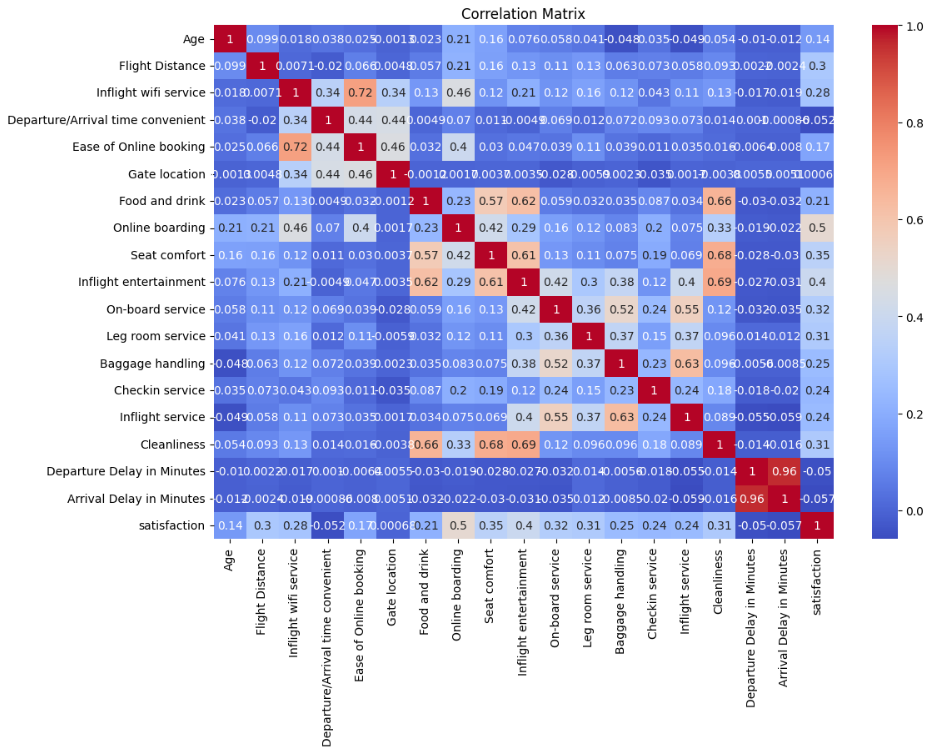
\includegraphics[width=0.9\linewidth, height=6cm]{1.png}
\caption{Covariance of variables}
\label{fig:subim2}
\end{subfigure}

\caption{Customer satisfaction data}
\label{fig:image2}
\end{figure}

From the plots we find that the variables are not uniformly distributed and there is multi-colinearity between these variables:

We must be cautious with these variables as they can cause errors in the model.\\
For processing these we removed some of the vectors that had high collinearity with others and also used \verb|StandardScaler| from the \verb|sci-kit library|. This is used to bring values from different columns into from whatever range they are in to a range of 0 to 1. This is important as higher values will cause heavy biasing.\\
Popular classical Machine learning algorithms from  the {\href{https://www.python.org/}{\texttt{Python}} library \href{https://scikit-learn.org/stable/index.html}{{\texttt{sklearn}}}} is used for model training and testing. From this library we will be using the \textbf{Logistic Regression model}, \textbf{Decision tree model},\textbf{Random forest },\textbf{SVM}
The performance evaluation of the models was done using their \textbf{Accuracy Score, Recall score and Precision score}. These scores are shown in the table below: 

\begin{center}
\label{tab:my-table1}
\begin{tabular}{|l|l|l|l|l|}
\hline
\begin{tabular}[c]{@{}l@{}}Model\\  No.\end{tabular} & Model Name               & Precision & Accuracy & Recall \\ \hline
1.                                                   & Logistic Regression      & 0.74     & 0.74    & 0.74  \\ \hline
2.                                                   & Decision tree & 0.92     & 0.92    & 0.92  \\ \hline
3.                                                   & Random forest      & 0.94751     & 0.94750    & 0.94541 \\ \hline
4.                                                   & SVM     & 0.95145    & 0.95146   & 0.95145  \\ \hline
\end{tabular}
    
\end{center}

\subsection{Confusion Matrix}
We can also use Confusion matrices to evaluate a model. The matrix of each model is given below.
\\The confusion matrix of the Logistic Regression model is shown below:
\begin{center}
   \includegraphics[width = 6cm]{2.png} 
\end{center}



The Logistic Regression model has 8826 True Negatives, 2887 False Positives, 2602 False negatives and 6466 True Positives \\

The confusion matrix of the Decision tree Classifier is shown below:\\
\begin{center}
        \includegraphics[width = 6cm]{3.png}
\end{center}



The Decision tree Classifier has 10903 True Negatives, 810 False Positives, 768 False negatives and 8300 True Positives \\

The confusion matrix of the Random forest is shown below:\\
\begin{center}
        \includegraphics[width = 6cm]{5.jpg}
\end{center}



The Decision tree Classifier has 0.54 True Negatives, 0.022 False Positives, 0.03 False negatives and 0.4 True Positives \\

The confusion matrix of the SVM is shown below:\\
\begin{center}
        \includegraphics[width = 6cm]{4.jpg}
\end{center}



The Decision tree Classifier has 0.55 True Negatives, 0.02 False Positives, 0.028 False negatives and 0.4 True Positives \\


\subsection{Future discussion}
This prediction model can be made more accurate with a dataset with more data and training the model on that would lead to more applications for the model.
More advanced models can be used to maximise the customer satisfaction.

\section{Conclusions}
The findings of this experiment effectively illustrated how machine learning models can be utilized to predict the customer's satisfaction by considering its  qualities. Through careful feature selection, thorough data analysis, and model training, we were able to generate dependable forecasts with noteworthy accuracy, with the Decision Tress Classifier emerging as the most suitable choice for this task. The insights garnered from this study have the potential to benefit the customer's satisfaction by enabling early quality evaluation and intervention techniques. To enhance prediction abilities further, future studies may explore the incorporation of new features or the utilization of more sophisticated algorithms. Taking everything into account, this research underscores the utility of machine learning in optimizing the customer satisfaction.\\
For further information and details of the project you can visit our \href{https://github.com/Christojs/IUFC-Project/blob/main/customer_satisfaction_prediction.ipynb}{{\texttt{GitHub Repository}}}

\section{Acknowledgments}
We extend our heartfelt gratitude and appreciation to Intel© Corporation for providing an invaluable opportunity to this project. First and foremost, we would like to express our sincere thanks to our team mentor Dr.Pradeep C for his unwavering guidance and constant support throughout the entirety of the project's development. Additionally, we are deeply indebted to our esteemed institution, Saintgits College of Engineering and Technology, for generously providing us with the necessary resources and facilitating sessions on essential topics such as machine learning. Furthermore, we extend our gratitude to all the pioneering researchers, scholars, and experts in the field of machine learning, natural language processing, and artificial intelligence, whose groundbreaking work has paved the way for the advancement of our project. We also acknowledge with appreciation the mentors, institutional heads, and industrial mentors for their invaluable guidance and support throughout the completion of this industrial training under the Intel© - Unnati Programme, whose expertise and encouragement have been instrumental in shaping our work and fostering our professional growth.
\section{Code discussion}
In the following section, we will provide concise explanations of the code used to create our model. While most of the code remains consistent throughout, variations primarily occur in the names of the models and their respective output variables.

\subsection{Code for Loading Required Libraries}
This is a very important step where we imported our required models, scalers, data processing libraries and performance measuring libraries.
\begin{lstlisting}[language=Python, caption=Libraries used]
import numpy as np
import pandas as pd
import matplotlib.pyplot as plt
import seaborn as sns
from sklearn.model_selection import train_test_split 
from sklearn.preprocessing import StandardScaler
from sklearn.ensemble import RandomForestClassifier
from sklearn.linear_model import LogisticRegression
from sklearn.linear_model import LinearRegression
from sklearn.cluster import KMeans
from sklearn.metrics import mean_squared_error
from sklearn.metrics import confusion_matrix
from sklearn.tree import DecisionTreeClassifier
from sklearn import metrics
\end{lstlisting}

\subsection{Data Pre-processing}
In this section we will handle the multi-colinearity and fit a classification model. This step also splits the data into training and testing set.
\begin{lstlisting}[language=Python]

%Assign X and y
df = pd.read_csv('data.csv')

# Drop non-numeric columns and convert 'satisfaction' to numeric
df_numeric = df.drop(['Gender', 'Customer Type', 'Type of Travel', 'Class'], axis=1)
df_numeric['satisfaction'] = df_numeric['satisfaction'].map({'neutral or dissatisfied': 0, 'satisfied': 1})

# Handling missing data
df_numeric.fillna(df_numeric.mean(), inplace=True)  # Replace NaN values with the mean of each column

# Split the data into features and target variable
X = df_numeric.drop('satisfaction', axis=1)
y = df_numeric['satisfaction']

# Split the data into training and testing sets
X_train, X_test, y_train, y_test = train_test_split(X, y, test_size=0.2, random_state=42)
\end{lstlisting}
The dataset is a clean and requires no further processing from here so we move on to model training and Evaluation.
We will evaluate the models based on accuracy, precision and recall scores.
\subsection{Model Training and Evaluation}
The only difference between the rest of the models and this one is the name of model imported from \verb|sci-kit learn|. So we will explain the basic procedure followed using this as an example. Initially we loaded the \verb|LogisticRegression| model trained it on our \verb|X_train and y_train| data and then used the \verb|.predict()| function to make a prediction using \verb|X_test|.The evaluation of the model is done using \verb|accuracy_score, precision_score, recall_score| functions available in \verb|sci-kit learn|.\\

\subsubsection{Logistic Regression }
We will create a Logistic Regression using available functions in scikit-learn. 
\begin{lstlisting}[language=Python]
lr = LogisticRegression()
lr.fit(X_train, y_train)
y_pred_lr = lr.predict(X_test)
print("Logistic Regression Classification Report:")
print(classification_report(y_test, y_pred_lr))
# Plot Logistic Regression Confusion Matrix
lr_cm = confusion_matrix(y_test, y_pred_lr)
plt.figure(figsize=(8, 6))
sns.heatmap(lr_cm, annot=True, cmap='Blues', fmt='g')
plt.xlabel('Predicted')
plt.ylabel('Actual')
plt.title('Logistic Regression Confusion Matrix')
plt.show()
\end{lstlisting}

\subsubsection{Decision Tree}
\begin{lstlisting}[language=Python]
dt = DecisionTreeClassifier()
dt.fit(X_train, y_train)
y_pred_dt = dt.predict(X_test)
print("Decision Tree Classification Report:")
print(classification_report(y_test, y_pred_dt))
# Plot Decision Tree Confusion Matrix
dt_cm = confusion_matrix(y_test, y_pred_dt)
plt.figure(figsize=(8, 6))
sns.heatmap(dt_cm, annot=True, cmap='Blues', fmt='g')
plt.xlabel('Predicted')
plt.ylabel('Actual')
plt.title('Decision Tree Confusion Matrix')
plt.show()
\end{lstlisting}







\subsubsection{Linear Regression }  We will create a Linear Regression using available functions in scikit-learn. 
\begin{lstlisting}[language=Python]
# Linear Regression
lr = LinearRegression()
lr.fit(X_train, y_train)
y_pred_lr = lr.predict(X_test)
print("Linear Regression Mean Squared Error:", mean_squared_error(y_test, y_pred_lr))
\end{lstlisting}


\section*{References}
\begin{itemize}
\item [1]Zhang Qiuyan, “Study on the customer satisfaction evaluation model and index system of the management consulting enterprises

,” IEEE Xplore,2012,doi: https://ieeexplore.ieee.org/document/6321227.
\item [2]Syanhrul Nizam Samsudin,and Bulan Abdullah, “Customer Satisfaction and Service Experience in Big Data Analytics for Automotive Service Advisor
,” IEEE Xplore,20222,doi: https://ieeexplore.ieee.org/document/9815482.

\item [3]Jianchi Xiang ,Xiaochang Chen, “Customer Satisfaction of E-Commerce Websites,” , Mar. 2009 International Workshop, doi: https://ieeexplore.ieee.org/abstract/document/5072797.
‌
\item [4]Motoi Iwashita, “Evaluating Customer Satisfaction with e-Books,” , Mar. 2015 International Workshop, doi: https://ieeexplore.ieee.org/abstract/document/7557781.
‌

\item [5]Pete Rotella and Sunita Chulani, “Analysis of customer satisfaction survey data,” , June . 2012 International Workshop, doi: https://dl.acm.org/doi/10.5555/2664446.2664459.
‌\end{itemize}
\end{document}
